\documentclass[
  captions=tableheading,
  bibliography=totoc, 
  titepage=firstiscover,
]{scrartcl}

\usepackage{blindtext} %neuer input

\usepackage{longtable} % Tabellen über mehrere Seiten

\usepackage[utf8]{inputenc} %neuer input

\usepackage{scrhack}

\usepackage[aux]{rerunfilecheck} %Warnung falls nochmal kompiliert werden muss

\usepackage{fontspec} %Fonteinstellungen

\recalctypearea{}

\usepackage[main=ngerman]{babel} %deutsche Spracheinstellung

\usepackage{ragged2e} %neuer input

\usepackage{amsmath, nccmath}

\usepackage{amssymb} %viele mathe Symbole

\usepackage{mathtools} %Erweiterungen für amsmath


\DeclarePairedDelimiter{\abs}{\lvert}{\rvert}
\DeclarePairedDelimiter{\norm}{\lVert}{\rVert}

\DeclarePairedDelimiter{\bra}{\langle}{\rvert}
\DeclarePairedDelimiter{\ket}{\lvert}{\rangle}

\DeclarePairedDelimiterX{\braket}[2]{\langle}{\rangle}{
#1 \delimsize| #2
}

\NewDocumentCommand \dif {m}
{
\mathinner{\symup{d} #1}
}


\usepackage[
  math-style=ISO,
  bold-style=ISO,
  sans-style=italic,
  nabla=upright,
  partial=upright,
  warnings-off={
    mathtools-colon,
    mathtools-overbracket,
  },
]{unicode-math}

\setmathfont{Latin Modern Math}
\setmathfont{XITS Math}[range={scr, bfscr}]
\setmathfont{XITS Math}[range={cal, bfcal}, StylisticSet=1]


\usepackage[
  locale=DE,
  separate-uncertainty=true,
  per-mode=reciprocal,
  output-decimal-marker={,},
]{siunitx}

\usepackage[autostyle]{csquotes} %richtige Anführungszeichen

\usepackage{xfrac}

\usepackage{float}

\floatplacement{figure}{htbp}

\floatplacement{table}{htbp}

\usepackage[ %floats innerhalb einer section halten
  section,   %floats innerhalb er section halten
  below,     %unterhalb der Section aber auf der selben Seite ist ok
]{placeins}

\usepackage[
  labelfont=bf,
  font=small,
  width=0.9\textwidth,
]{caption}

\usepackage{subcaption} %subfigure, subtable, subref

\usepackage{graphicx}

\usepackage{grffile}

\usepackage{booktabs}

\usepackage{microtype} %Verbesserungen am Schriftbild

\usepackage[
backend=biber,
]{biblatex}

\addbibresource{../lit.bib}

\usepackage[ %Hyperlinks im Dokument
  german,
  unicode,
  pdfusetitle,
  pdfcreator={},
  pdfproducer={},
]{hyperref}

\usepackage{bookmark}

\usepackage[shortcuts]{extdash}

%\usepackage{warpcol}

\usepackage{physics}
\allowdisplaybreaks

\begin{document}
    \title{Physik IV Übungsblatt 9}
    \author{  
    Tobias Rücker\\
    \texorpdfstring{\href{mailto:tobias.ruecker@tu-dortmund.de}{tobias.ruecker@tu-dortmund.de}
    \and}{,} 
    Paul Störbrock\\
    \texorpdfstring{\href{mailto:paul.stoerbrock@tu-dortmund.de}{paul.stoerbrock@tu-dortmund.de}}{}
    }
\maketitle
\center{\Large Abgabegruppe: \textbf{4H}}
\thispagestyle{empty}

\newpage
\tableofcontents
\thispagestyle{empty}
\newpage

\setcounter{page}{1}

\section{Aufgabe 1}

    \begin{figure}[H]
        \centering
        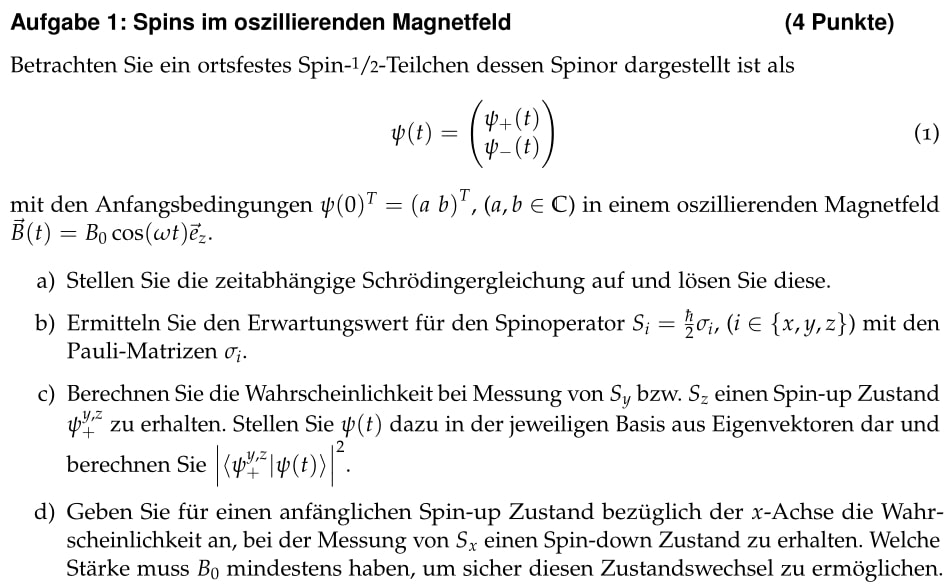
\includegraphics[width=\textwidth]{images/Aufgabe1.jpg}
        \label{fig:1}
    \end{figure}

\subsection{a)}

\subsection{b)}

\subsection{c)}

\subsection{d)}

\section{Aufgabe 2}

    \begin{figure}[H]
        \centering
        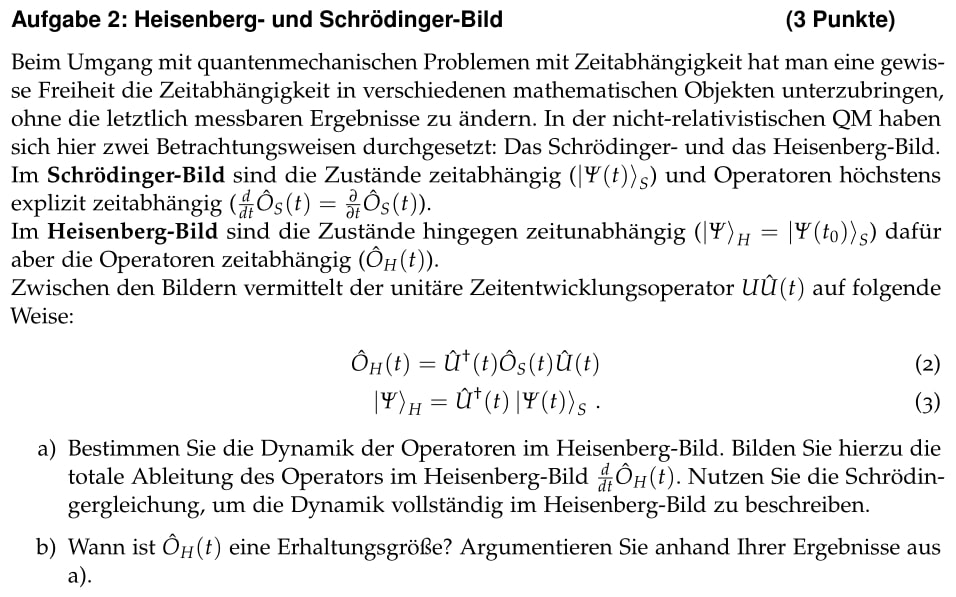
\includegraphics[width=\textwidth]{images/Aufgabe2a.jpg}
        \label{fig:2}
    \end{figure}

    \begin{figure}[H]
        \centering
        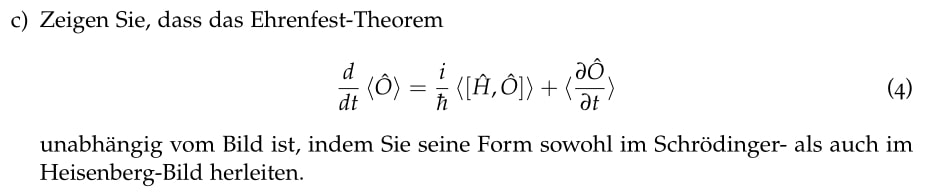
\includegraphics[width=\textwidth]{images/Aufgabe2b.jpg}
        \label{fig:3}
    \end{figure}

\subsection{a)}

\subsection{b)}

\subsection{c)}

\section{Aufgabe 3}

    \begin{figure}[H]
        \centering
        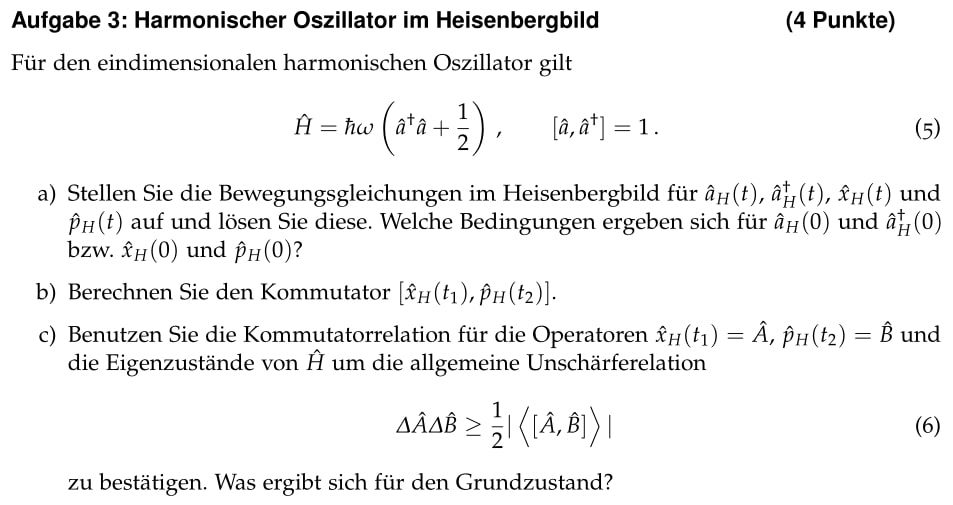
\includegraphics[width=\textwidth]{images/Aufgabe3.jpg}
        \label{fig:4}
    \end{figure}

\subsection{a)}

\subsection{b)}

    \begin{align*}
        \left[ \hat{x}_H(t_1),\hat{p}_H(t_2) \right] &= x_s e^{i\omega t_1} \cdot p_s e^{i\omega t_2} - p_s e^{i\omega t_2} \cdot x_s e^{i\omega t_1}\\
        &= x_s p_s e^{i\omega t_1} e^{i\omega t_2} - p_s x_s e^{i\omega t_2} e^{i\omega t_1}\\
        &= e^{i\omega (t_1+t_2)} (x_s \cdot p_s - p_s \cdot x_s)\\
        &= e^{i\omega (t_1+t_2)}[x_s,p_s]\\
        [x_s,p_s] &= \sqrt{\frac{\hbar}{2m\omega}}i \sqrt{\frac{m\omega\hbar}{2}} \underbrace{[a+a^{\dagger},a^{\dagger}-a]}_{=1+1=2}\\
        &= i\frac{\hbar}{2} \cdot 2 = i\hbar\\
        \Rightarrow \left[ \hat{x}_H(t_1),\hat{p}_H(t_2) \right] &= i\hbar e^{i\omega (t_1+t_2)}
    \end{align*}

\subsection{c)}

    \begin{align*}
        \Delta \hat{A} \Delta \hat{B} \leq \frac{1}{2} \abs{\langle \left[ \hat{A},\hat{B} \right] \rangle}\\
        \Delta A &= \langle (A-\langle A \rangle )^2 \rangle\\
        &= \bra{Y} \left( A-\langle A \rangle \right)^2 \ket{Y}\\
        &= \bra{Y} \left( A-\langle A \rangle \right)\left( A-\langle A \rangle \right) \ket{Y}\\
        &= \braket{f}{f}\\
        \Delta B &= \langle (B-\langle B \rangle )^2 \rangle\\
        &= \bra{Y} \left( B-\langle B \rangle \right)^2 \ket{Y}\\
        &= \bra{Y} \left( B-\langle B \rangle \right)\left( B-\langle B \rangle \right) \ket{Y}\\
        &= \braket{g}{g}\\
        \Delta A \Delta B &= \braket{f}{f} \braket{g}{g}
        \intertext{
            \flushleft{Zwischenrechnung:\;}\justifying
        }
        \braket{f}{g} &= \bra{Y} \left( A-\langle A \rangle \right)\left( B-\langle B \rangle \right) \ket{Y}\\
        &= \bra{Y} \left( AB - A\langle B\rangle - \langle A\rangle B + \langle A\rangle \langle B\rangle  \right) \ket{Y}\\
        &= \langle A\rangle \langle B\rangle - \langle B\rangle \langle A\rangle - \langle A\rangle \langle B\rangle + \langle B\rangle \langle A\rangle\\
        &= \langle A\rangle \langle B\rangle - \langle A\rangle \langle B\rangle\\
        \braket{g}{f} &= \bra{Y} \left( B-\langle B \rangle \right)\left( A-\langle A \rangle \right) \ket{Y}\\
        &= \bra{Y} \left( BA - B\langle A\rangle - \langle B\rangle A + \langle B\rangle \langle A\rangle  \right) \ket{Y}\\
        &= \langle B\rangle \langle A\rangle - \langle A\rangle \langle B\rangle - \langle B\rangle \langle A\rangle + \langle A\rangle \langle B\rangle\\
        &= \langle B\rangle \langle A\rangle - \langle B\rangle \langle A\rangle
        \intertext{
            \flushleft{Ende\;}\justifying Zwischenrechnung
        } 
        \braket{f}{g} - \braket{g}{f} &= \langle A\rangle \langle B\rangle - \langle B\rangle \langle A\rangle = \left[ \langle A\rangle, \langle B\rangle \right]
    \end{align*}

\section{Aufgabe 4}

    \begin{figure}[H]
        \centering
        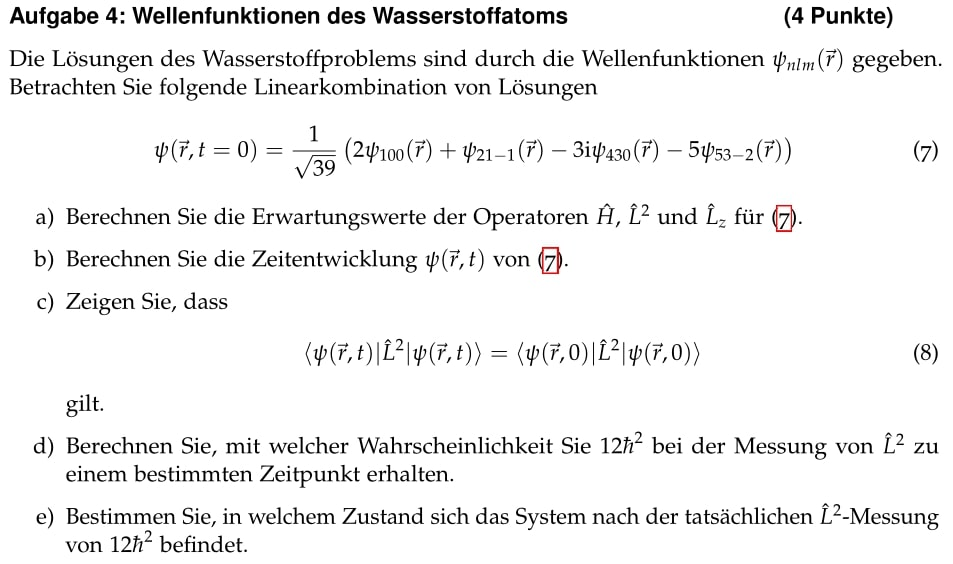
\includegraphics[width=\textwidth]{images/Aufgabe4.jpg}
        \label{fig:5}
    \end{figure}

\subsection{a)}

    \begin{align*}
        \langle \hat{L}^2 \rangle &= \int \Psi^*\left( \vec{r},t=0 \right) \hat{L}^2 \Psi\left( \vec{r},t=0 \right)\\
        &= \frac{1}{39} \int \left( 2\Psi_{100} + \Psi_{21-1} - 3\Psi_{430} - 5\Psi_{53-2} \right)^* \cdot \hat{L}^2 \left( 2\Psi_{100} + \Psi_{21-1} - 3i\Psi_{430} - 5\Psi_{53-2} \right)\\
        &= \frac{1}{39} \int \left( 2\Psi_{100}^* + \Psi_{21-1}^* + 3i\Psi_{430}^* - 5\Psi_{53-2}^* \right) \hbar^2 \left( 2\Psi_{21-1} - 36i\Psi_{430} - 60\Psi_{53-2} \right)\\
        &= \hbar^2 \frac{1}{39} \left( \int 2\abs{\Psi_{21-1}}^2 + \int 108\abs{\Psi_{430}}^2 + \int 300\abs{\Psi_{53-2}}^2 \right)\\
        &= \frac{410}{39} \hbar^2\\
        \\
        \langle \hat{L}_z \rangle &= \int \Psi^*(\vec{r},t=0) \hat{L}_z \Psi(\vec{r},t=0)\\
        &= \frac{1}{39} \int \left( 2\Psi_{100} + \Psi_{21-1} - 3i\Psi_{430} - 5\Psi_{53-2} \right)^* \hat{L}_z \left( 2\Psi_{100} + \Psi_{21-1} - 3i\Psi_{430} - 5\Psi_{53-2} \right)\\
        &= \frac{1}{39} \int \left( 2\Psi_{100}^* + \Psi_{21-1}^* + 3i\Psi_{430}^* - 5\Psi_{53-2} \right) \left( -\hbar\Psi_{21-1} + 10\hbar\Psi_{32-2} \right)\\
        &= -\frac{51}{39} \hbar\\
        \\
        \langle \hat{H} \rangle &= \int \Psi^*(\vec{r},t=0) \hat{H} \Psi(\vec{r},t=0)\\
        &= \frac{1}{39} \int \left( 2\Psi_{100} + \Psi_{21-1} - 3i\Psi_{430} - 5\Psi_{53-2} \right)^* \hat{H} \left( 2\Psi_{100} + \Psi_{21-1} - 3i\Psi_{430} - 5\Psi_{53-2} \right)\\
        &= \frac{1}{39} \int \left( 2\Psi_{100}^* + \Psi_{21-1}^* + 3i\Psi_{430}^* + 5\Psi_{53-2}^* \right) \left( 2E_{100}\Psi_{100} + E_{21-1}\Psi_{21-1} + 3iE_{430}\Psi_{430} - 5E_{53-2}\Psi_{53-2} \right)\\
        &= \frac{1}{39} \left( 4E_{100} + E_{21-1} - 9E_{430} + 25E_{53-2} \right)
    \end{align*}

\subsection{b)}

    \begin{align*}
        \hat{H} \ket{E_{lmn}} &= E_{lmn} \ket{E_{lmn}}\\
        \ket{\Psi_{lmn}} &= \sum_{lmn} \alpha_{lmn}(t) \ket{E_{lmn}}
        \intertext{
            \flushleft{Zeitabhängige\;}\justifying Schrödingergleichung:
        }
        i\hbar\partial_t \ket{\Psi} &= \hat{H} \ket{\Psi}\\
        i\hbar\partial_t \ket{\Psi} &= \hat{E}_{lmn} \ket{\Psi}\\
        \Rightarrow \sum_{lmn} i\hbar\partial_t \left( \alpha_{lmn}(t)\ket{E_{lmn}} \right) &= \sum_{lmn} \alpha_{lmn}(t) E_{lmn} \ket{E_{lmn}}\\
        \sum_{lmn} \left( \underbrace{i\hbar \dot{\alpha}_{lmn} E_{lmn}}_{=0,\;\text{da $E_{lmn}$ lin.unabh.}} \ket{E_{new}} \right)\\
        0 &= i\hbar \dot{\alpha}_{lmn} - \alpha_{lmn} E_{lmn}\\
        \Leftrightarrow \dot{\alpha} &= -\frac{E_{lmn}}{\hbar} i \alpha_{lmn}\\
        \alpha_{lmn}(t) &= \alpha_{lmn}(0)\exp(-E_{lmn}i)\\
        \alpha_{lmn}(0) &= \langle E_{lmn} \abs{\Psi(0)} \rangle
        \intertext{
            \flushleft{Es\;}\justifying bleibt nur der Term mit gleichen Indizes über, da die Indizes ansonsten null sind.
            Die Vorfaktoren in Gl. 7 sind $\alpha_{lmn}(0)$:
        }
        \Psi(\vec{r},t) &= \frac{1}{\sqrt{39}} ( 2\Psi_{100}(\vec{r}) \exp\left( -\frac{E_{100}}{\hbar}it \right)\\
         &+ \Psi_{21-1}(\vec{r}) \exp\left( -\frac{E_{21-1}}{\hbar}it \right)\\
         &+ 3i\Psi_{430}(\vec{r}) \exp\left( -\frac{E_{430}}{\hbar}it \right)\\
         &- 5\Psi_{53-2} \exp\left( -\frac{E_{53-2}}{\hbar} it \right) )
    \end{align*}

\subsection{c)}

    \begin{align*}
        \bra{\Psi(\vec{r},0)} \hat{L}^2 \ket{\Psi(\vec{r},0)} &= \frac{410}{39} \hbar^2\\
        \bra{\Psi(\vec{r},t)} \hat{L}^2 \ket{\Psi(\vec{r},t)} &= \frac{1}{\sqrt{39}} \int ( 2\Psi_{100}(\vec{r}) \exp\left( -\frac{E_{100}}{\hbar} it \right)\\
        &+ \Psi_{21-1}(\vec{r}) \exp\left( -\frac{E_{21-1}}{\hbar} it \right)\\
        &+ 3i\Psi_{430}(\vec{r}) \exp\left( -\frac{E_{430}}{\hbar} it \right)\\
        &- 5\Psi_{53-2}(\vec{r}) \exp\left( -\frac{E_{53-2}}{\hbar} it \right) )^* \hat{L}^2 ( 2\Psi_{100} \exp\left( -\frac{E_{100}}{\hbar} it \right)\\
        &+ \Psi_{21-1}(\vec{r}) \exp\left( -\frac{E_{21-1}}{\hbar} it \right)\\
        &+ 3i\Psi_{430}(\vec{r}) \exp\left( -\frac{E_{430}}{\hbar} it \right)\\
        &- 5\Psi_{53-2}(\vec{r}) \exp\left( -\frac{E_{53-2}}{\hbar} it \right) )\\
        \\
        &= \frac{1}{\sqrt{39}} \int ( 2\Psi_{100}^*(\vec{r}) \exp\left( \frac{E_{100}}{\hbar} it \right)\\
        &+ \Psi_{21-1}^*(\vec{r}) \exp\left( \frac{E_{21-1}}{\hbar} it \right)\\
        &+ 3i\Psi_{430}^*(\vec{r}) \exp\left( \frac{E_{430}}{\hbar} it \right)\\
        &- 5\Psi_{53-2}^*(\vec{r}) \exp\left( \frac{E_{53-2}}{\hbar} it \right) ) \hbar^2 (\\
        &+ 2\Psi_{21-1}(\vec{r}) \exp\left( -\frac{E_{21-1}}{\hbar} it \right)\\
        &+ 36i\Psi_{430}(\vec{r}) \exp\left( -\frac{E_{430}}{\hbar} it \right)\\
        &- 60\Psi_{53-2}(\vec{r}) \exp\left( -\frac{E_{53-2}}{\hbar} it \right) )\\
        &= \frac{410}{39}\hbar^2
    \end{align*}

\subsection{d)}

    \flushleft{Bestimmter\;}\justifying Zeitpunkt $t=0$:
    \begin{align*}
        12\hbar^2 \qquad m=3\\
        \braket{\Psi_{l3n}}{\Psi(\vec{r},t=0)} &= \frac{9}{39} + \frac{25}{39} = \frac{34}{39} = \text{\SI{87.18}{\percent}}
        \intertext{
            \flushleft{Es\;}\justifying besteht eine Wahrscheinlichkeit von \SI{87.18}{\percent} um im Zeitpunkt $t=0$ $12\hbar^2$ zu erhalten.
        }
    \end{align*}

\subsection{e)}

\end{document}